\section{Implementation}\label{sec:impl}

Our \tube system has two components; the tube itself and the screen. As shown in Figure~\ref{fig:impl1}, the tube is attached to an acrylic enclosure that houses a small Force-Sensing Resistor (FSR) and Inertial Measurement Units (IMU) that possesses 5 degree of freedom from 3-axis accelerometer and 2-axis gyroscope. The IMU captures the 3-dimensional motions of the tube and translate it into 2-dimensional position on the screen using basic kinematics manipulation and euler's discretization method. Additionally, it also records the angle in which the tube is rotated and how fast it is rotating. With the FSR integrated in the tube, how hard the user breathe into the tube is also captured. All of these informations will then be passed into arduino which will be read by a processing module.

\begin{figure}
  \centering
  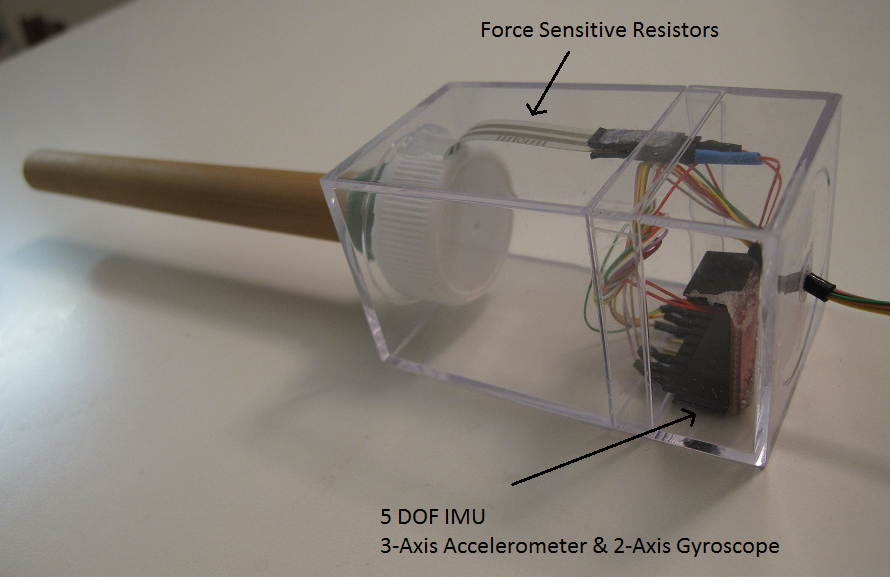
\includegraphics[width=\linewidth]{./figs/impl1.png}
  \caption{Our \tube with all the sensors.}
  \label{fig:impl1}
\end{figure}

Figure~\ref{fig:design-sketch} shows an overview of how our \tube system works in a whole. As we move or rotate \tube, our movements are recorded by an Arduino microcontroller. Arduino will then send all of the data it received to be used by the applications in the computer.

\begin{figure}
  \centering
  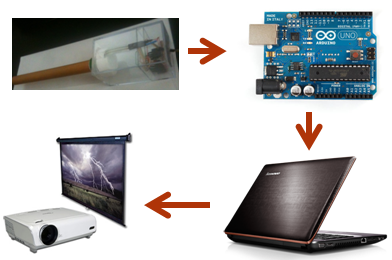
\includegraphics[width=0.8\linewidth]{./figs/sketch.png}
  \caption{Overview of how our system works.}
  \label{fig:design-sketch}
\end{figure}

We have developed two applications to demonstrate the uniqueness and interactiveness of our \tube. The applications that we developed are written in processing since it provides a smooth interface with Arduino while boasting numerous easy-to-use graphical functions. Making existing processing applications to work with our \tube require very minimal changes to the existing code base since we have made the interface to the hardware to be very simple and generic.

\subsection{\textbf{Painting Application}}

Our first application is a painting application program. In this application, the user will be able to paint by blowing into the tube and the harder the user blows, the thicker the color is. Changing the color of the paint is achieved by rotating the tube. We implement the paint to be brush-like and the color will disappear after a while to make it more like painting with a real brush.

\begin{figure}
  \centering
  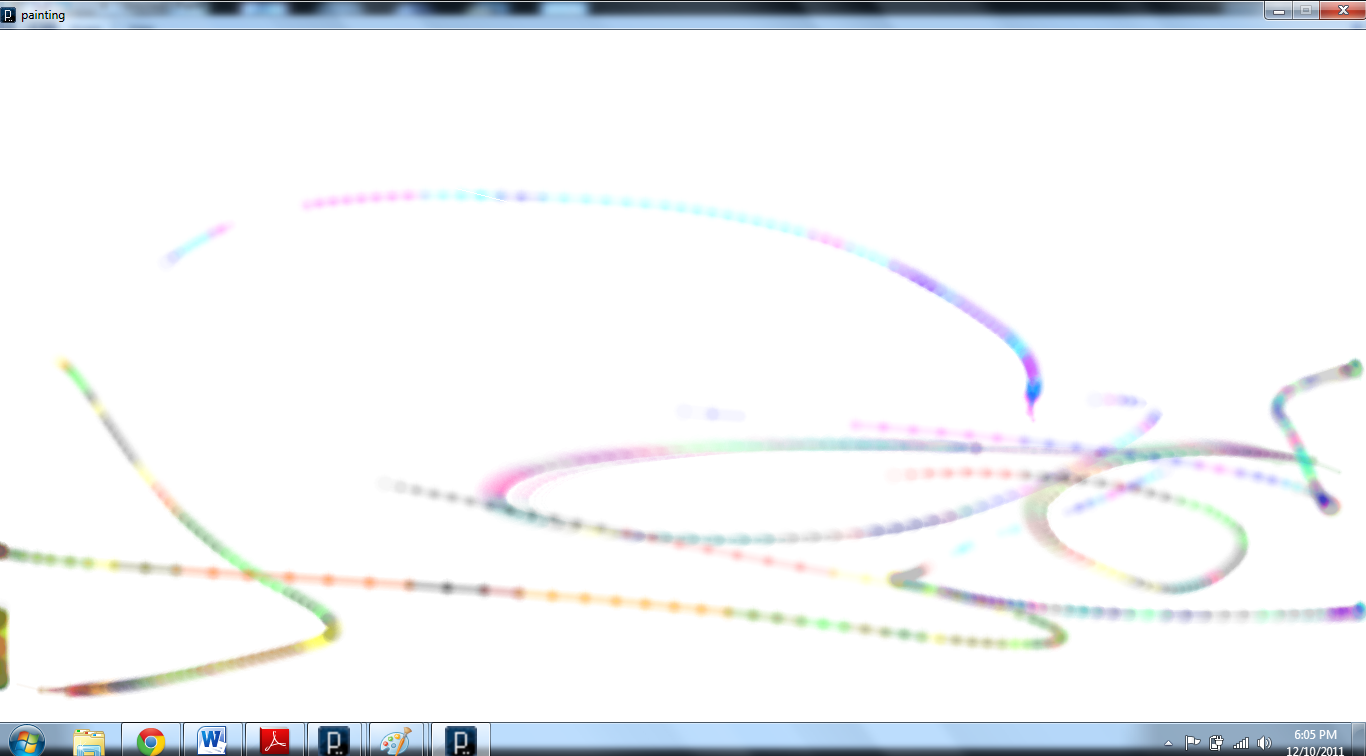
\includegraphics[width=\linewidth]{./figs/tube3.png}
  \caption{A screenshot of our painting application that one of our testers draws.}
  \label{fig:painting}
\end{figure}

\subsection{\textbf{Balloon Popping Game}}

The next application that we developed is a game in which the user is required to pass through a set of levels by shooting down balloons that randomly appear in the screen, as shown Figure~\ref{fig:shooting-game}. This is done by moving the pointer to where the balloons are and blow into the tube. The game consists of two levels: stage 1 and stage 2. In the first stage, the pointer and the balloons' color are always black so that users don’t have to rotate the tube to match the color. This stage is intended to familiarize the users with the basic concept on controlling the movement of our \tube to pop a balloon. In the second stage, the balloons are randomly generated with red, green, or blue color and the users will have to rotate the tube to match the color of the pointer with the color of the balloon before being able to pop the balloon.

\begin{figure}
  \centering
  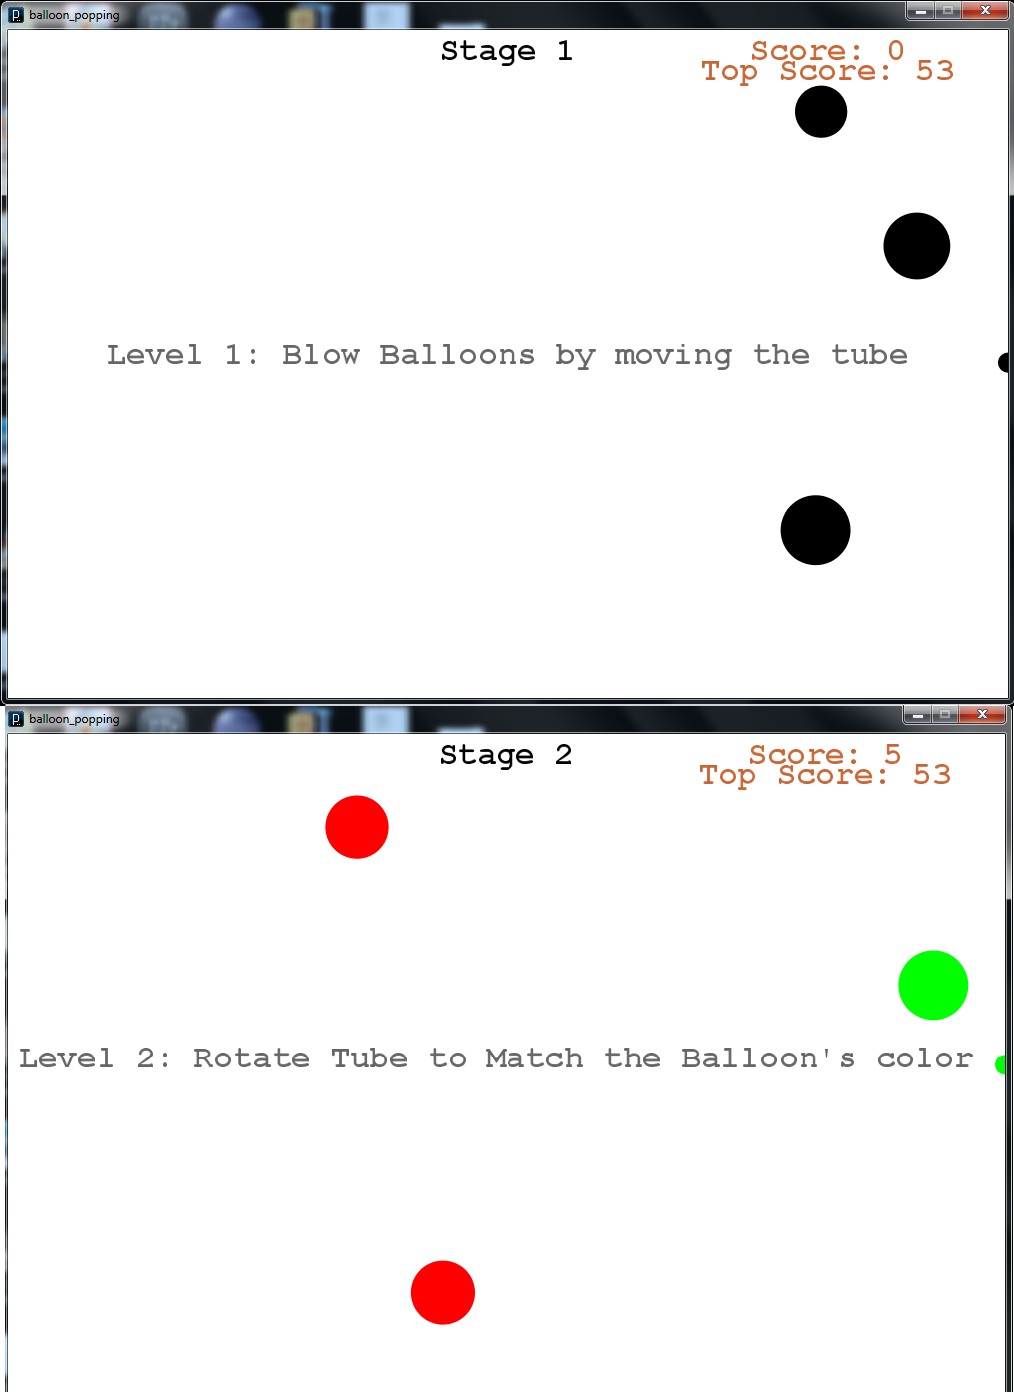
\includegraphics[width=0.70\linewidth]{./figs/tubemaster.png}
  \caption{A screenshot of the beginning of each level of our balloon popping game.}
  \label{fig:shooting-game}
\end{figure}
